\chapter{Realizability}
\label{chap:realizability}

\section{Basic definitions}
\label{sec:basic-definitions}

\subsection{Motivation and the basic idea}
\label{sec:realizability-basic-idea}

Realizability was introduced by Stephen Kleene~\cite{KleeneSC:intint}
who used it to build a model of intuitionistic arithmetic. Our purpose
is to study not only the theoretical aspects of computable
mathematics, but also practical issues. Thus we approach realizability
by asking a practical question: given a mathematical structure
(constants, functions, relations, and axioms), what should a computer
implementation look like? For simple cases, the answer is obvious. A
group would have a type whose values represent group elements, a value
representing the neutral element, and functions which compute the
group operation and inverses. But for more interesting structures,
especially those arising in mathematical analysis, the answer is less
clear. How do we implement the real numbers (and we do not mean
floating-point arithmetic, we mean the \emph{real} real numbers)?
Which operations on a compact metric space can be implemented? How do
we implement a space of smooth functions? Significant research goes
into finding satisfactory answers to such
questions~\cite{Wei00,TZ98,Bla97}.

To explain the basic idea behind realizability we consider a small
real-world programming example. Suppose we are asked to design a data
structure for the set $\mathsf{Graphs}$ of all finite
simple\footnote{Simple means at most one arrow between any two
  vertices.} directed graphs with vertices labeled by distinct
integers. An typical such graph~$G$ is shown in
Figure~\ref{fig:digraph}.
%
\begin{figure}[htp]
  \centering
  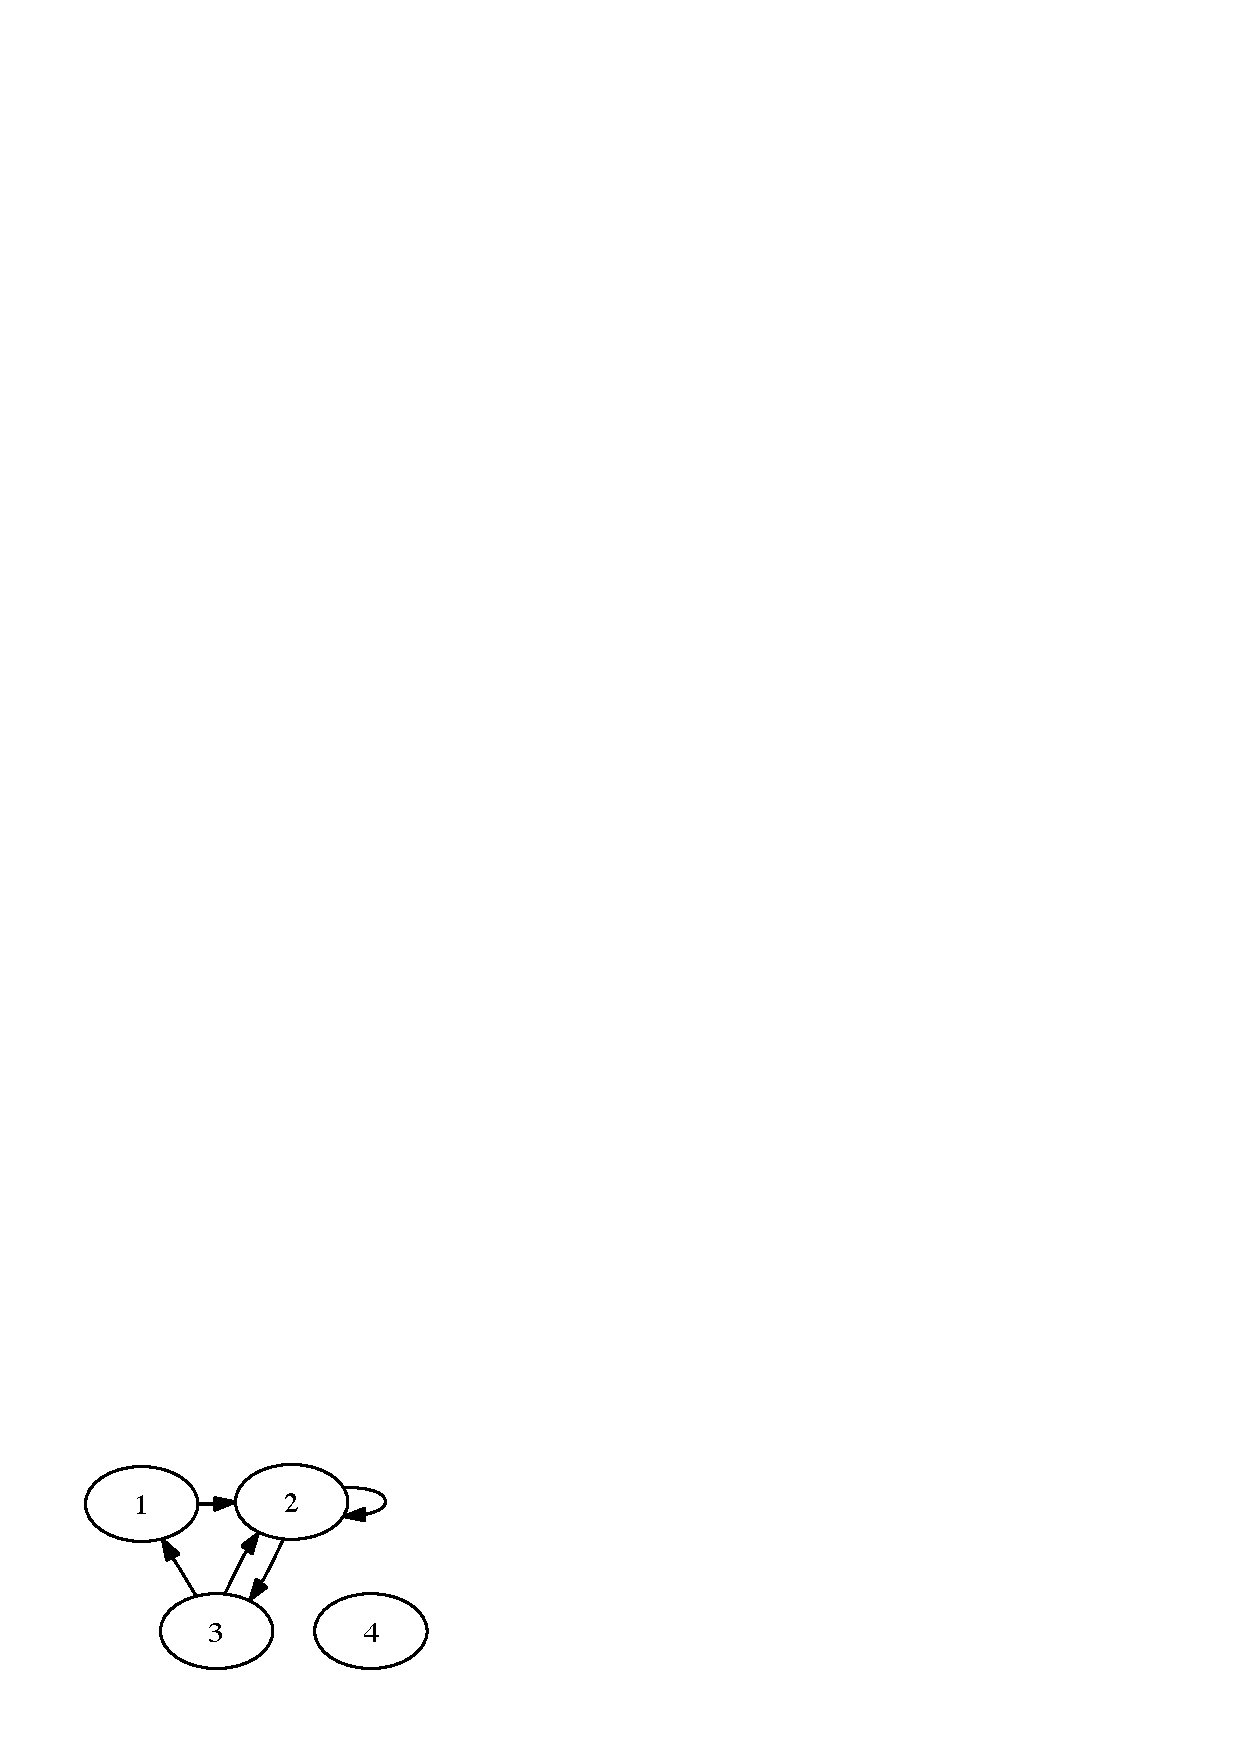
\includegraphics[width=0.3\textwidth]{digraph}
  \caption{A finite directed graph $G$}
  \label{fig:digraph}
\end{figure}
%
One common representation of such graphs uses a pair of lists
$(\ell_V, \ell_A)$, where $\ell_V$ is the list of vertex labels and
$\ell_A$ is the \emph{adjacency list} representing the arrows by
pairing the labels of each source and target. For the above graph $G$,
$\ell_V = [1, 2, 3, 4]$ and $\ell_A = [(1,2), (2,2), (2,3), (3,2),
(3,1)]$.
%
Thus we define the datatype of graphs as\footnote{We use Haskell
  notation in which $[t]$ is the type of lists of elements of
  type~$t$, and $(t_1, t_2)$ is the cartesian product of types~$t_1$
  and~$t_2$.}
%
\begin{lstlisting}[language=Haskell]
type Graph = ([Int], [(Int, Int)])
\end{lstlisting}
%
However, this is not a complete description of the intended
representation, as there are representation invariants and conditions
not expressed by the type, e.g.,
%
\begin{enumerate}
\item The order in which vertices and arrows are listed is not
  important%
; for example, $[1,2,3,4]$ and $[4,1,2,3]$ represent the same vertices.
\item Each vertex and arrow must be listed exactly once.
\item The source and target of each arrow must appear in the list of vertices.
\end{enumerate}
%
Consequently, to fully implement the mathematical
set~$\mathsf{Graphs}$ we must not only decide on the underlying
datatype $\mathtt{graph}$, but also determine what values of that type
represent which elements of~$\mathsf{Graphs}$. All this can be
expressed with a \emph{realizability relation}
%
\begin{equation*}
  r \rz x
\end{equation*}
%
which is read as ``$r$ realizes $x$''. In the above example we would
write
%
\begin{equation*}
([1, 2, 3, 4], [(1,2), (2,2), (2,3), (3,2), (3,1)]) \rz G.
\end{equation*}
%
Once the set $\mathsf{Graphs}$ is implemented as a datatype, an
obvious thing to do is to compute with it. When can we say that a
function $f : \mathsf{Graphs} \to \mathsf{Graphs}$ is computable? The
answer again is quite natural for a programmer: $f$ is computed by a
program $p : \mathtt{graph} \to \mathtt{graph}$ when $p$ does to
realizers what $f$ does to elements: if $r \rz G$ then $p(r) \rz
f(G)$. We say that the map $f$ is \emph{realized} or \emph{tracked} by
the program~$p$.


\subsection{Assemblies}
\label{sec:assemblies}

We now give a precise definition of the ideas presented in the
previous section.

\begin{definition}[Assemblies]
  Let $A$ be a TPCA and $\comp{A}$ a sub-TPCA. An \emph{assembly}
  over~$(A, \comp{A})$ is a triple $(S, |S|, {\rz_S})$ where $S$ is a
  set, $|S|$ is a type, and $\rz_S$ is a relation between $A_{|S|}$
  and~$S$ satisfying: for every $x \in S$ there is $r \in A_{|S|}$
  such that $r \rz_S x$.

  A \emph{realized map} $f : S \to T$ between assemblies $(S, |S|,
  {\rz_S})$ and $(T, |T|, {\rz_T})$ is a map for which there exists $p
  \in \comp{A}_{|S| \to |T|}$ satisfying: if $r \rz_S x$ then $\defined{p
    \cdot r}$ and $p \cdot r \rz_T f(x)$.
\end{definition}

\noindent
By a traditional abuse of notiation we shall often denote an assembly
$(S, |S|, {\rz_S})$ simply as~$S$.

There are many versions of realizability. Ours is known as \emph{typed
  relative realizability}. It is typed because we used typed PCAs
rather than the ordinary ones. It is relative because we used one
TPCA~$A$ for assemblies, and another for the realized maps. By this we
are capturing the idea that computable functions may operate on
potentially non-computable data, as was the case for type~2 machines
and the graph model, cf.\ Sections~\ref{sec:type-2}
and~\ref{sec:graph-model}. In the typical case the larger TPCA~$A$
allows representation of arbitrary data, but the sub-TPCA $\comp{A}$
consists only of the computable part of~$A$ which forces the realizers
for maps to be computable. Thus it makes sense to say in the general
case that the maps are realized \emph{relative} to the choice of a
sub-TPCA~$\comp{A}$.

When $A$ is not typed the definition of an assembly simplifies a bit
because we need not keep mentioning the (trivial) types: an assembly
over a PCA~$A$ is a pair $(S, {\rz_S})$ where $S$ is a set and $\rz_S$
is a relation between~$A$ and~$S$, such that for every $x \in S$ there
is $r \in A$ and $r \rz_S x$.

Another special case occurs when $\comp{A} = A$. In this case we write
$\Asm{A}$ instead of $\Asm{A,A}$.

In most examples the TPCA $A$ is actually an NR-TPCA, and $\comp{A}$ a
sub-NR-TPCA of~$A$.

Particular choices of a TPCA with sub-TPCA yield well known ``schools
of computable mathematics'':
%
\begin{enumerate}
\item When $A = \comp{A} = \NN$ is the first Kleene algebra we get the
  Russian school of \emph{recursive
    mathematics}~\cite{recursive-math}, also known as \emph{type I
    computability} because the underlying computational model is that
  of type~1 machines.
\item When $A = \Baire$ is the second Kleene algebra we get Kleene's
  \emph{function realizability}~\cite{KleeneSC:fouim}, also known by
  its newer name \emph{type two effectivity (TTE)}~\cite{tte}. There
  are actually three variants:
  %
  \begin{enumerate}
  \item $A = \comp{A} = \Baire$ is \emph{continuous} function
    realizability because maps are realized by arbitrary continuous
    realizers,
  \item $A = \Baire$ and $\comp{A} = \comp{\Baire}$, where
    $\comp{\Baire}$ is the set of computable sequences, is the
    \emph{relative} type 2 realizability,
  \item $A = \comp{A} = \comp{\Baire}$ is the \emph{computable}
    function realizability.
  \end{enumerate}
  %
  We will mostly study the continuous and the relative function
  realizaiblity.
\item When $A = \Scott$ is the graph model we get a version of
  realizability that is closely related to equilogical
  spaces~\cite{BauerA:equs}. Here two there are three variants:
  %
  \begin{enumerate}
  \item $A = \comp{A} = \Scott$ is the continuous model,
  \item $A = \Scott$ and $A = \comp{\Scott}$ is the family of
    c.e.~sets is the relative model,
  \item $A = \Scott = \comp{\Scott}$ is the computable model.
  \end{enumerate}
\item Closely related to the previous case is $A = U$ where~$U$ is a
  universal Scott domain~\cite{GunterScott}. This again gives as three
  variants of \emph{domain representations}~\cite{Bla97,Bla97a}.
\item The case $A = \PCFinf$ and $\comp{A} = \PCF$ was used by
  Mart{\'\i}n Escard\'o in his investigations of compact, exhausitble
  and searchable sets~\cite{Escardo}.
\end{enumerate}
%
In Section~\ref{variants} we shall study some of these in greater
detail.


\begin{proposition}
  Assemblies and realized maps form the \emph{category
    $\Asm{A,\comp{A}}$ of assemblies over $(A, \comp{A})$}.
\end{proposition}

\begin{proof}
  If $f : S \to T$ and $g : T \to U$ are realized by $q \in A_{|S| \to
    |T|}$ and $r \in A_{|T| \to |U|}$, respectively, then their
  composition $g \circ f$ is realized by
  $\pcalam{\annot{x}{|S|}}{r\,(q\,x)} =
  \combS\,(\combK\,r)\,(\combS\,(\combK\,q)\,(\combS\,\combK\,\combK))$.
  The identity map $\id_S : S \to S$ is realized by
  $\pcalam{\annot{x}{|S|}}{x} = \combS\,\combK\,\combK$. Composition
  is associative because it is just composition of maps.
\end{proof}

\subsection{Sets as assemblies}
\label{sec:nabla}

Suppose $(S, |S|, {\rz_S})$ is an assembly over $(A, \comp{A})$. The
only requirement for the realizability relation $\rz_S$ is that every
$x \in S$ be realized by some $r \in A_{|S|}$. In particular,
different elements of~$S$ are allowed to share the same realizer.
The extreme case, in which all elements share all realizers, 

Let $t$ be a type such that $A_t$ is inhabited. Such a type always
exists, because there is some type $s$, and then $t = s \to s \to s$
contains $\combK_{s,s}$. Given any set $X$, let $\nabla X = (X, t,
{\rz_{\nabla X}})$ be the assembly whose underlying set is~$X$ and the
realizability relation is trivial, i.e., $r \rz_{\nabla X} x$ for all
$x \in X$ and $r \in A_t$. If $f : X \to Y$ is any map between
sets~$X$ and~$Y$ then~$f$ is a morphism $\nabla f : \nabla X \to
\nabla Y$ because it is tracked by $\pcalam{\annot{x}{t}}{x}$. This
defines a functor
%
\begin{equation*}
  \nabla : \Set \to \Asm{A,\comp{A}}.
\end{equation*}
%
Up to natural isomorphism, $\nabla$ is independent of the choice of
type~$t$. We will study the properties of $\nabla$ later on. For now
we notice that $\nabla$ is full and faithful, which means that
$\Asm{A,\comp{A}}$ contains the category of sets as a full
subcategory.

\subsection{Modest sets}
\label{sec:modest-sets}

The functor $\nabla$ is devoid of any computational content because it
represents a set~$X$ by a trivial realizability relation which conveys
no information at all about the elements of~$X$. Consequently, we
cannot compute anything interesting regarding~$X$. It is useful to
impost a further restriction on the realizability relations which
prevents such anomalies.

\begin{definition}
  An assembly $(S, |S|, {\rz_S})$ is \emph{modest} when each $r \in
  A_{|S|}$ realizes at most one element of~$S$. A modest assembly is
  also called a \emph{modest set}.
\end{definition}

\noindent
In symbols, modesty is the property
%
\begin{equation*}
  \xall{r}{A_{|S|}}{
    \all{x,y}{S}{
      r \rz_S x \land r \rz_S y \implies x = y
    }
  }.
\end{equation*}
%
The full subcategory of $\Asm{A,\comp{A}}$ of the modest sets is
denoted by~$\Mod{A, \comp{A}}$. The terminology was suggested by Dana
Scott because the cardinality of modest sets does not exceed the
cardinality of the TPCA~$A$.



\section{Equivalent formulations}
\label{sec:equivalent-formulations}

\subsection{Existence predicates}
\label{sec:existence-predicates}

\subsection{Partial equivalence relations}
\label{sec:pers}

\subsection{Representations}
\label{sec:representations}

\section{Schools of Computabile Mathematics}
\label{sec:schools}

\subsection{Recursive Mathematics}
\label{sec:recursive-math}

\subsection{Type Two Effectivity}
\label{sec:tte}

% Admissibility.

\subsection{Equilogical spaces}
\label{sec:equilogical-spaces}

\subsection{Domain representations}
\label{sec:domain-representations}



%%% Local Variables: 
%%% mode: latex
%%% TeX-master: "notes"
%%% End: 
